\section{Testing Framework}

The testing framework developed for this project plays a pivotal role in validating the functionality and accuracy of the beat detection algorithm. A robust testing script is integral to this process, enabling the automated comparison of BPM estimates produced by our algorithm against those generated by the external tool bpm-tools. The bpm-tools, developed by Mark Hills\footnote{Mark Hills - bpm-tools project website: \url{http://www.pogo.org.uk/~mark/bpm-tools/}}, serve as a valuable benchmark for assessing the accuracy of our implementation. The bpm-tools project is released under the GPLv2 license (December 2021)\footnote{GPLv2 License - \url{http://www.gnu.org/licenses/old-licenses/gpl-2.0.html}}.

\subsection{Preparation of Test Audio Files}

Prior to executing the testing script, it is crucial to prepare the audio files to ensure consistency and compatibility. This preparation involves two essential steps: converting FLAC files to WAV format and trimming WAV files to a uniform length.

\subsubsection{Converting FLAC to WAV}

The script \texttt{flac2wav.sh} is used to convert FLAC files to WAV format, which is necessary for the beat detection algorithm to have a uniform input format. To execute the conversion, follow these steps:

\lstset{style=ShellStyle}
\begin{lstlisting}[caption={Converting FLAC to WAV}, label=lst]
./flac2wav.sh path/to/flac_files_directory
\end{lstlisting}

\subsubsection{Trimming WAV Files}

The \texttt{cutWAVs.sh} script trims WAV files to the first 30 seconds to standardize the duration of audio samples for testing. This ensures that the BPM analysis is performed under consistent conditions across all test files. To use cutWAVs.sh, navigate to the testing directory and execute the script.

\lstset{style=ShellStyle}
\begin{lstlisting}[caption={Trimming WAV Files}, label=lst]
./cutWAVs.sh path/to/wav_files_directory
\end{lstlisting}

\subsection{Testing Script Usage}

After preparing the audio files, the testing script automates the evaluation process across these files. The script is designed to be executed in a Unix shell. Navigate to the \texttt{src/testing} directory and execute:

\lstset{style=ShellStyle}
\begin{lstlisting}[caption={Executing the Testing Framework}, label=lst]
./testBulk.sh path/to/wav_files_directory
\end{lstlisting}

This script processes each WAV file in the specified directory, comparing our BPM estimate with that obtained from \texttt{bpm-tools}. The results are compiled into \texttt{output\_table.txt}, including the song name, our BPM estimate, and the \texttt{bpm-tools} estimate.

Additionally, \texttt{testBulk.sh} calls \texttt{plot\_bland\_altman.m}, generating a Bland-Altman plot that visually compares our BPM estimates against those from \texttt{bpm-tools}. This plot provides a graphical representation of the agreement between the two sets of BPM values, highlighting any systematic bias or variability.

\subsection{Test Cases and Methodology}

The framework was applied to Tidal's Top 100 Germany tracks, providing a diverse range of genres and tempos for comprehensive evaluation. This diversity ensures that the testing encompasses a wide range of musical characteristics, challenging the algorithm's versatility and accuracy.

\subsection{Statistical Analysis and Visualization}

After running the \texttt{testBulk.sh} script to analyze Tidal's Top 100 tracks, we used statistical analysis and a Bland-Altman plot to evaluate the performance of our beat detection algorithm compared to \texttt{bpm-tools}. The statistical analysis showed that our algorithm detected an average BPM of 133.49, while bpm-tools detected an average of 121.313 BPM. The algorithm detected a median BPM value of 140, while \texttt{bpm-tools} detected a median BPM value of 122.846. The median relative difference between the two values was 3.96\%, indicating a high degree of alignment in performance. Any minor discrepancies are likely due to differences in the algorithmic approaches used for BPM detection.

To visually assess the agreement between the two BPM detection methods and explore any systematic bias or variability, a Bland-Altman plot was generated. This plot displays the average BPM (calculated as the mean of the BPM values from our algorithm and \texttt{bpm-tools} for each track) on the x-axis against the relative difference (our BPM minus \texttt{bpm-tools}' BPM, relative to \texttt{bpm-tools}' BPM) on the y-axis. This visualization aids in identifying any consistent bias in our algorithm's BPM detection relative to \texttt{bpm-tools}, as well as the variability of this difference across the range of average BPMs.

\begin{figure}[H]
\centering
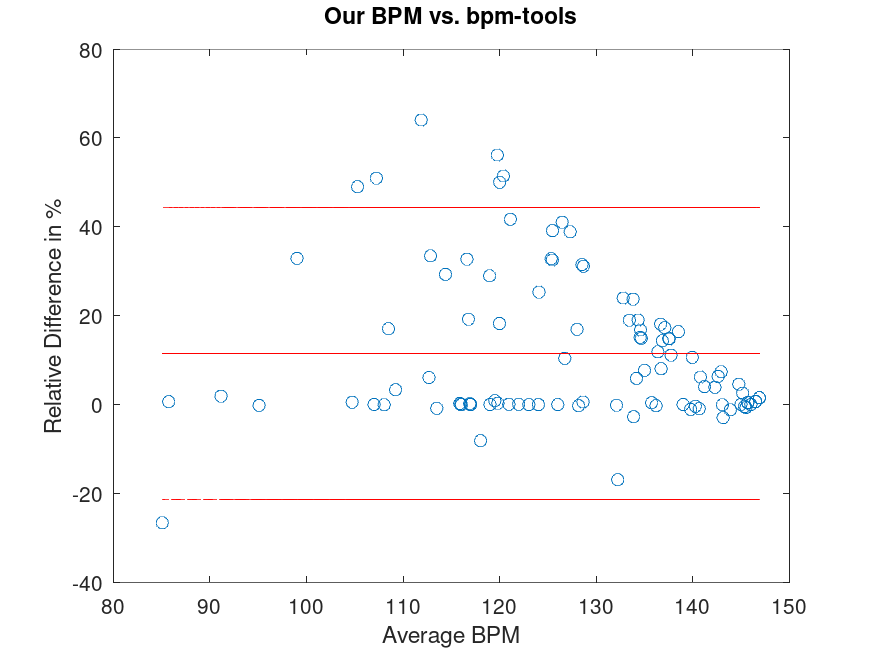
\includegraphics[width=0.8\textwidth]{bland_altman_plot.png}
\caption{Bland-Altman Plot visualizing the agreement between our BPM detection and \texttt{bpm-tools}.}
\end{figure}

The analysis using Bland-Altman plot shows interesting trends in the performance of our beat detection algorithm compared to bpm-tools, especially when the BPM values are close to 150. The convergence towards bpm-tools' estimates around the 150 BPM mark can be attributed to the configuration of our algorithm's EXPECTED\_BPM parameter, which is set at 150. This setting affects the calculation of minimum samples between beats, directly impacting the accuracy of detected BPM values in this range.   Adjusting the EXPECTED\_BPM parameter may optimize performance across a broader range of BPM values.

It is important to note that bpm-tools, while highly regarded, is not infallible. A comprehensive evaluation of our algorithm's effectiveness would require a comparison against a robust and validated BPM database. Unfortunately, such a comparison was beyond the scope of this project's timeline. Efforts to facilitate this comparison are underway. Ongoing work is being done to secure API access to a suitable BPM database. This future work promises to provide a more detailed assessment of our beat detection algorithm's accuracy and reliability across a wide range of musical genres and BPMs.

\subsection{Conclusion}

The testing framework has proven to be indispensable in assessing the accuracy and reliability of the beat detection algorithm through its comprehensive and automated approach. It enables a nuanced understanding of the algorithm's performance by facilitating direct comparison with established benchmarks, guiding ongoing development efforts, and ensuring robustness across a diverse musical spectrum.
